\documentclass{article}
\usepackage[T1]{fontenc}
\usepackage{lmodern}
\usepackage{graphicx}
\usepackage{amsmath,amssymb}
\usepackage[a4paper,margin=2cm]{geometry}
\usepackage[absolute,overlay]{textpos}
\setlength{\TPHorizModule}{1mm}
\setlength{\TPVertModule}{1mm}
\usepackage[indonesian]{babel}
\usepackage{hyperref}
\setlength{\emergencystretch}{2em}
% unit: Halaman 21

\begin{document}

% === Halaman 21 (python/native) ===

• Hasil ekspansi, yaitu E(Ri – 1) di-XOR-kan dengan 

Ki menghasilkan blok A berukuran 48-bit:


E(Ri – 1)  Ki = A 

• Blok A dikelompokkan menjadi 8 kelompok, 

masing-masing 6 bit, dan menjadi masukan bagi 

proses substitusi. 

• Ada 8 matriks substitusi, masing-masing 

dinyatakan dengan kotak-S.

• Kotak –S menerima masukan 6 bit dan 

memberikan luaran 4 bit.

21

% deskripsi: gambar native xref 116
\noindent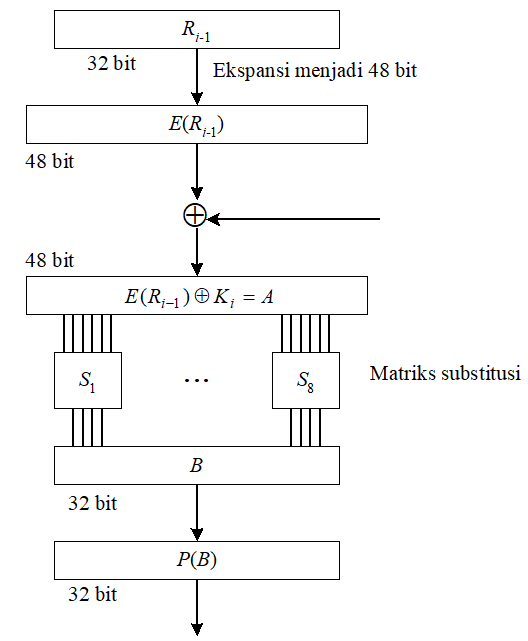
\includegraphics[width=0.85\textwidth]{../../images/python/page_021_img_01.png}

\end{document}
